% Requires running Bibtex

\documentclass[%
reprint,
amsmath,amssymb,
aps,
floatfix
]{revtex4-2}

\usepackage{graphicx}% Include figure files
\usepackage{dcolumn}% Align table columns on decimal point
\usepackage{bm}% bold math
\usepackage{hyperref}% add hypertext capabilities
\usepackage[font=scriptsize,labelfont=bf, justification=justified]{caption}% change fontsize in captions
\usepackage{float}
\usepackage{booktabs}% cool table style
\hypersetup{
	colorlinks=true,       % false: boxed links; true: colored links
	linkcolor=black,        % color of internal links
	citecolor=black,        % color of links to bibliography
	filecolor=black,     % color of file links
	urlcolor=black         
}

\usepackage{listings}

%\usepackage{bibspacing}
%\setlength{\bibitemsep}{.5\baselineskip plus .05\baselineskip minus .05\baselineskip}


\begin{document}
	
	\preprint{APS/123-QED}
	
	\title{PHYC30170 Physics with Astronomy and Space Science Lab 1;\\An Investigation into Compton Scattering}
	
	\author{Daragh Hollman}
	\email{daragh.hollman@ucdconnect.ie}
	
	\date{\today}
	
	\begin{abstract}
		The aim of this report was to investigate the scattering interaction between gamma rays and electrons known as Compton scattering. The aims were to determine the energy of the gamma ray after the interaction as a function of angle and to determine the differential cross-section. This was done by studying the gamma ray energy spectrum of a gamma emitting Caesium-137 source after scattering off an aluminium sample. A separate experiment was undertaken to investigate whether the electrons in this interaction needed to be treated relativistically or if classical assumptions were sufficient. The energy spectrum and differential cross-section as a function of scattering angle were determined and it was concluded that the electrons should be treated relativistically.
	\end{abstract}

	\maketitle
	
	\section{Introduction}
	Compton scattering is the interaction in the collision of a gamma ray with a free electron \cite{manual1}. In this interaction the gamma ray imparts some of its energy to the electron as it scatters away at an angle. It is important to understand how gamma rays interact with other particles, and Compton scattering is one of the tools which helps to bring about that understanding. Compton scattering has many applications in radiobiology, biomedical science, and in astrophysics \cite{KURODA2011S183}\cite{harding}\cite{alessia} including x-ray imaging and the study of active galactic nuclei.
	
	\section{Energy and Cross-Section Determination}
	
		\subsection{Theory}
		
			\subsubsection{Energy Determination}		
			The Compton scattering interaction can be described with the same kinematic equations that describe the collision of two balls in a game of snooker \cite{manual1}. The interaction is shown in figure \ref{fig:diagram}. An incoming gamma ray (photon) of energy $E_\gamma$ collides with an electron at rest which results in the gamma being scattered off with reduced energy $E_{\gamma'}$ at some angle $\theta$, imparting kinetic energy to the electron. The electron gains energy $E_e$ and it itself scatters at an angle $\phi$.\\
			
			The energy of the gamma ray after scattering can be calculated using the principles of the conservation of energy and momentum. By the conservation of energy the energy of the incident gamma ray  is equal to the energy of the scattered gamma ray and the kinetic energy of the scattered electron, we have:
			\begin{equation}
				E_\gamma = E_{\gamma'} + E_e
			\end{equation}
			
			Similarly, by the conservation of momentum, the momentum of the incident gamma ray is equal to the momentum of the scattered components. This can be broken up into the components along each axis as follows. In the x direction we have:
			\begin{equation}
				\frac{hf}{c} = \underbrace{\frac{hf'}{c} \cos{\theta}}_\text{scattered gamma ray} + \underbrace{mv \cos{\phi}}_\text{scattered electron}
			\end{equation}and in the y direction with zero initial momentum we have:
			\begin{equation}
				0 = \underbrace{\frac{hf}{c} \sin{\theta}}_\text{scattered gamma ray} - \underbrace{mv \sin{\phi}}_\text{scattered electron}
			\end{equation}Note that as $E_\gamma = hf$ we also have $E_{\gamma'} = hf'$, and that $m$ represents the relativistic mass of the electron, $m = \gamma m_0$, where here $m_0$ is the rest mass of the electron and $\gamma$ represents the Lorentz factor, $\gamma = \left( 1 - \frac{v^2}{c^2} \right)^{-1/2}$.\\
			
			These three equations can be solved to give an equation for the energy of the scattered gamma ray, $E_{\gamma'}$, in terms of the incident gamma ray energy, $E_\gamma$, the rest mass energy o the electron, $m_0 c^2$, and the scattering angle, $\theta$ \cite{manual1}.
			\begin{equation}
				E_{\gamma'} = \frac{E_\gamma}{1 + \frac{E_\gamma}{m_0 c^2} \left( 1 - \cos{\theta} \right)}
			\end{equation}We know the electron rest mass to be $m_0 c^2 = 0.511 \,\text{MeV}$ and we know that the gamma rays from the Caesium-137 source used in this experiment have energy $0.662 \,\text{MeV}$. As as a result of this, we can represent the energy of the scattered gamma ray in terms of the scattering angle only. We find that:
			\begin{equation}
				\frac{1}{E_{\gamma'}} = 1.51 + 1.956 \left( 1 - \cos{\theta} \right)
				\label{eq:inverseGammaEnergyTheory}
			\end{equation}and hence it is clear that the inverse of the energy of the scattered ray has a linear relationship with one minus the cosign of the angle it scattered at.\\
			
			\subsubsection{Cross-Section Determination}
			The differential cross-section is the fraction of the total number of scattered particles that emerge from a solid angle \cite{fowler}. In Compton scattering, the differential cross-section is the probability for each angle that an incident gamma ray is scattered \cite{manual1}. The Klein-Nishina formula is an equation of the differential cross-section treated quantum mechanically \cite{yazaki}. In a simplified (classical) form we have equations \ref{eq:klein-nishina},
			\begin{widetext}
			\begin{equation}
				\frac{d\sigma}{d\Omega} = \frac{r_0}{2}\left( \frac{1 + \cos^2 \theta}{\left[1 + \alpha (1-\cos\theta)\right]^2} \right) \times \left( 1 + \frac{\alpha^2 (1-\cos\theta)^2}{(1 + \cos^2 \theta)(1 + \alpha[1 - \cos\theta])} \right)
				\label{eq:klein-nishina}
			\end{equation}
			\end{widetext}measured in $\text{cm}^2 / \text{sr}$ where $r_0$ is the classical electron radius, $\alpha = \frac{E_\gamma}{m_0 c^2}$, and $d\Omega$ is the solid angle in steradians. The differential cross-section can also be represented in the measurable quantities in this experiment:
			\begin{equation}
				\frac{\partial \sigma}{\partial \Omega} = \frac{\Sigma_{\gamma'}}{N \Delta \Omega I}
			\end{equation}where $\Sigma_{\gamma'}$ is the sum under the photopeak divided by the counting time and the intrinsic peak efficiency, $N$ is the number of electrons in the scattering sample, $\Delta \Omega$ is the solid angle of the detector, and $I$ is the number of incident gamma rays per unit area per second at the scattering sample.\\
			
			Therefore, in this experiment we will measure the energy of the scattered gamma ray for many different scattering angles and scatter the inverse of the energy against $(1-\cos\theta)$. Using a linear least squares fit to these points we can directly compare the result against the theoretical linear result in equation \ref{eq:inverseGammaEnergyTheory}. We will also use the net counts for each angle to determine the differential cross-section and compare it to the Klein-Nishina formula, eq \ref{eq:klein-nishina}.

			\begin{figure}
				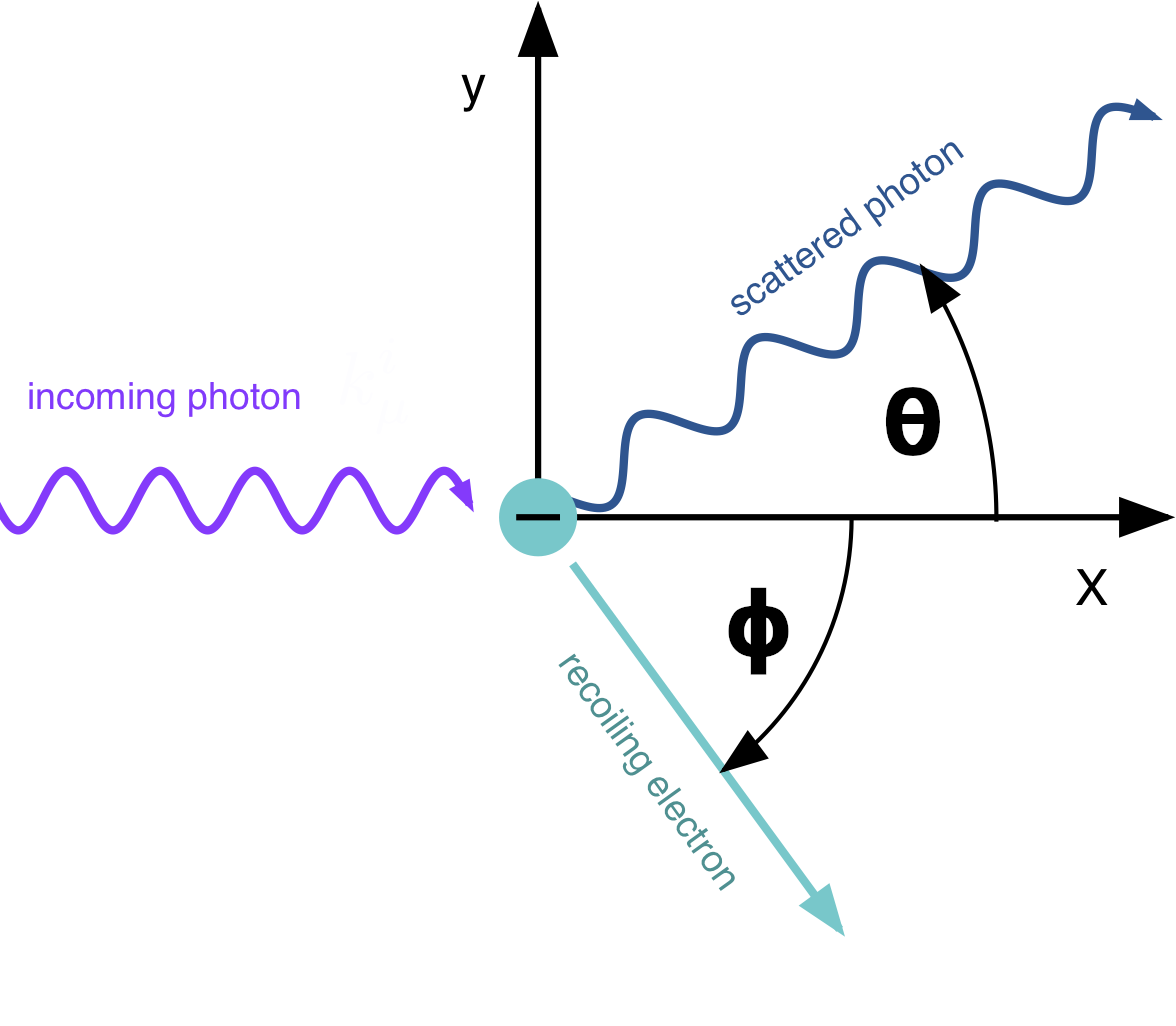
\includegraphics[width=0.7\columnwidth]{compton_scattering.png}
				\caption{\label{fig:diagram}A diagram of the Compton scattering interaction \cite{comptonFIU}. A photon is scattered off an electron with a transfer of energy.}
			\end{figure}
		
		\subsection{Methodology}
					
			\subsubsection{Apparatus}			
			
			The apparatus was set up as shown in figure \ref{fig:apparatus1}. A thallium-activated sodium iodide detector (NaI(Tl)) and a photomultiplier tube were used to detect the gamma rays. This detector was placed inside of a lead shielding which was on rails free to rotate 100 degrees either side of the axis of the emitter and the scattering sample. Electrons in the detector crystal are excited by the gamma rays and the scintillations produced from the return to ground state are detected and produced as signals by a photomultiplier tube. The electronics were turned on prior to taking measurements to allow them to approach working temperature.\\
			
			\begin{figure}
				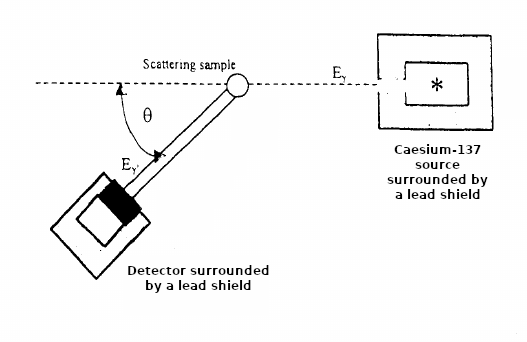
\includegraphics[width=0.85\columnwidth]{apparatus1.png}
				\caption{\label{fig:apparatus1}A schematic of the apparatus used \cite{manual1}.}
			\end{figure}					
			
			A source of Caesium-137 was used as the gamma ray emitter. This source was encased in lead shielding with a closable opening on the side facing towards the detector and scattering sample. A cylinder of aluminium was chosen to be the scattering sample.
			
			\subsubsection{Calibration}			
			
			MAESTRO Multichannel Analyser Emulation Software was used to analyse the energy spectrum. Before measurements could be made using the apparatus, the software had to be calibrated to determine the energy at each channel. To do this, two small calibration sources with known gamma ray energy were placed directly in front of the detector so that the rays would arrive directly (no scattering). The two calibration substances used were Caesium-137 and Americium-241, with gamma ray energies of $662 \,\text{keV}$ and $59.5 \,\text{keV}$ respectively. Using more calibration sources would increase the accuracy of the calibration, however for the purposes of this experiment, the reduction in uncertainty because of this would be insignificant compared to other uncertainties due to the Gaussian nature of the photopeak and the uncertainty on the angle.\\
			
			\subsubsection{Data Collection}			
			
			Starting from perpendicular to the axis of emission, data were taken in 5 degree steps between 90 and 20 degrees from the emission axis. Angles lower than 20 degrees were not usable as some gamma rays would arrive at the detector unscattered and hence interfere with the analysis. The angles were measured by taking the left and right side of the detector mount on the graduated rail and determining the midpoint. The uncertainty on this measurement was determined to be 0.25 degrees based on half the resolution of the graduation however, as there existed some imprecision in the positioning of the detector in its housing, a more lenient approximation of the uncertainty on the angle of 2 degrees was taken.\\
			
			The spectrum recorded is similar to that shown in figure \ref{fig:gammaSpectrum}. Measurements of the photopeak Gaussian were taken from the minimum point between the Compton edge and the photopeak to the end of the high energy tail of the Gaussian of the photopeak. To calculate the net counts, the software assumes a linear transition between this minimum and this gaussian tail to account for multiple scattering occurrences. The angle, photopeak energy, photopeak FWHM, net counts (including uncertainty) and the live time were all recorded in appendix A.
			
			\begin{figure}
				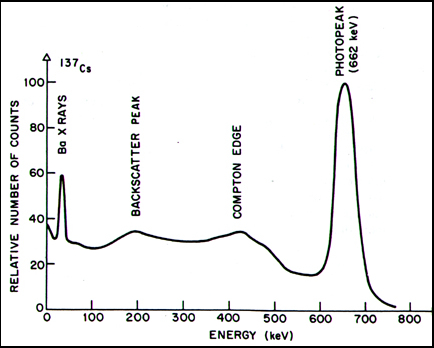
\includegraphics[width=0.85\columnwidth]{gammaspectrum.jpg}
				\caption{\label{fig:gammaSpectrum}The spectrum observed from a typical Caesium-137 source \cite{vcu}.}
			\end{figure}
		
		\subsection{Results and Analysis}
			The reciprocal of the energy of the scattered gamma ray was plotted against the angle in figure \ref{fig:energyPlot}. A linear least squares fit was applied and compared to the theory. Note that as the data contained both an uncertainty in the x and y directions an orthogonal distance regression would in theory be a more accurate fit, however as the x uncertainties were mostly insignificant compared to the y uncertanties, for simplicity a least squares fitting was used instead. The fitted line has a slope of $1.93$ with an intercept of $1.57$. We see a slight offset from the from the theory line in figure \ref{fig:energyPlot} however the slope is very similar. This is likely due to a systematic error in the alignment of the apparatus such as a misalignment of the placement of the detector in its housing. The total uncertainties for this data were determined by propagating the error on the measured values through their respective equations.\\
			
			\begin{figure}
				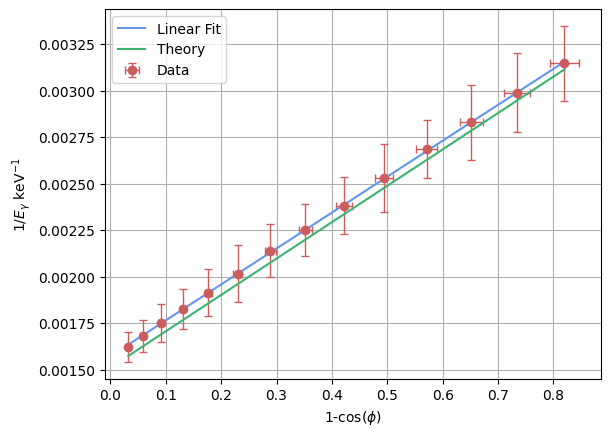
\includegraphics[width=0.85\columnwidth]{energyPlot.png}
				\caption{\label{fig:energyPlot}A scatter plot of the data with a fitted line. This is compared to the theory of equation \ref{eq:inverseGammaEnergyTheory}.}
			\end{figure}
			
			The total net counts under the photopeak were divided by the counting time and plotted against the scattering angle in figure \ref{fig:crossSectionPlot}, and compared to the Klein-Nishina formula. We see that, as predicted, that the low angle data points deviate from the theory. This is due to the unwanted inclusion of direct gamma rays arriving at the detector unscattered. The data in this plot was initially much lower than the theory values (however still of the same order). The data was multiplied by a constant scalar of 4.95 to match the theoretical line. This was determined visually. This constant offset is likely due to an inaccurate assumption of the activity of the source included in the calculations. The source used is old and would have decayed multiple half-lives since the measurement was taken. Again the total uncertainties for this plot were determined by propagating the error on the measured values through their respective equations.\\
			
			\begin{figure}
				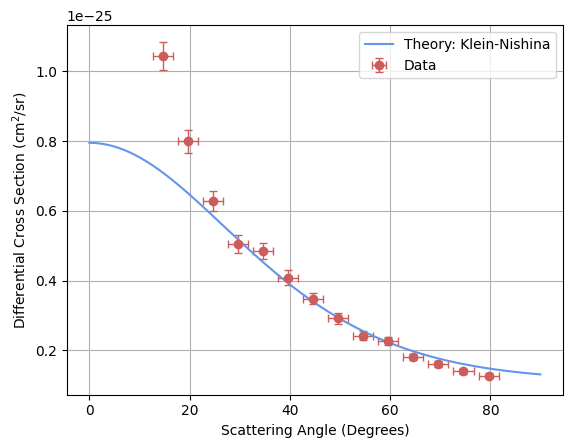
\includegraphics[width=0.85\columnwidth]{crossSectionPlot.png}
				\caption{\label{fig:crossSectionPlot}A scatter plot of the data comparing the measured cross-section to the theoretical values calculated by the Klein-Nishina equation, equation \ref{eq:klein-nishina}.}
			\end{figure}
		
	\section{Relativity and the Electron Rest Mass}	
		
		\subsection{Theory}
			In the previous section we assumed that the electrons involved in the scattering process needed to be treated relativistically. We know this must be true as our data follows closely that of the theory, however, this can be tested more rigorously by determining the rest mass of the electron. This can be done by comparing the kinetic energy of the electron and the energy of the scattered gamma ray.\\
			\subsubsection{Classical Calculation}
			Similarly to section II.A we must consdier the conservation of energy and momentum in the collision. We know the classical relation between the energy and momentum of a photon to be $E_\gamma = p_\gamma c$. The Compton edge of the gamma ray energy spectrum in figure \ref{fig:gammaSpectrum} represents the incident gamma ray being backscattered, i.e. a scattering angle of 180 degrees. Hence by conservation of momentum we have \cite{manual2}:
			\begin{equation}
				p_\gamma = p - p_\gamma '
			\end{equation}where $p_\gamma$, $p$, and $p_\gamma '$ are the momenta of the incident gamma ray, the electron after scattering, and the scattered gamma ray respectively. By conservation of energy we have:
			\begin{equation}
				p_\gamma c = p_\gamma 'c + T
			\end{equation}where T is the kinetic energy of the electron. These two equations can be combined to yield an expression for the total energy in terms of the measurable quantities.
			\begin{equation}
				pc = 2 E_\gamma - T
			\end{equation}\\
			
			In the classical approach, we take the non-relativistic kinetic energy, $T = p^2 / 2m_{nr}$, were the mass subscript corresponds to the non-relativistic mass. Hence we can substitute the momentum into this expression to find the rest mass of the electron in terms of the measurable quantities.
			\begin{equation}
				m_{nr} = \frac{p^2 c^2}{2T} = \frac{(2 E_\gamma - T)^2}{2T}
				\label{eq:classical}
			\end{equation}
			
			\subsubsection{Relativistic Calculation}
			Factoring for special relativity we have the total electron energy equalling the rest mass energy and the kinetic energy,
			\begin{equation}
				p^2 c^2 + (m_0 c^2)^2 = (T + m_0 c^2)^2 = E_e^2
			\end{equation}yielding the energy-momentum relationship for special relativity \cite{manual2}. We can then relate the rest mass in terms of the measurable quantities:
			\begin{equation}
				m_0 c^2 = \frac{p^2 c^2 - T^2}{2T} = \frac{2 E_\gamma (E_\gamma -T)}{T}
				\label{eq:relativistic}
			\end{equation}
		
		Therefore, by plotting the equations for the classical rest mass and the relativistic rest mass (equations \ref{eq:classical} and \ref{eq:relativistic} respectively) and comparing the two, we can see whether the electrons in this reaction need to be treated relativistically.		
		
		
			% These figures are placed earlier as Latex's float placing algs need more time for a full width.
			\begin{figure}
				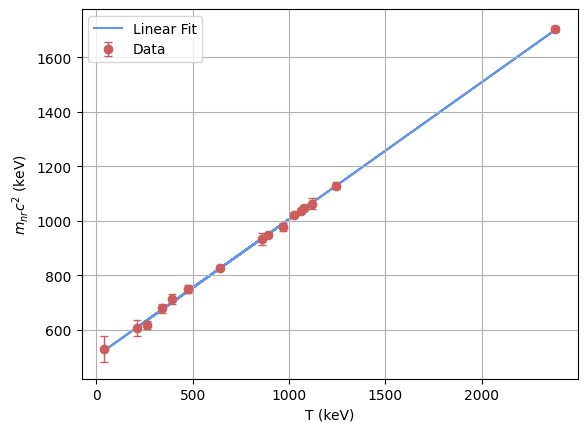
\includegraphics[width=0.85\columnwidth]{classicalRestMass.png}
				\caption{\label{fig:classicalRestMass}A graph of the calculations for $mc^2$ using the energies measured from the sources. We see that the rest mass energy increases as a function of kinetic energy.}
			\end{figure}

			\begin{figure*}
				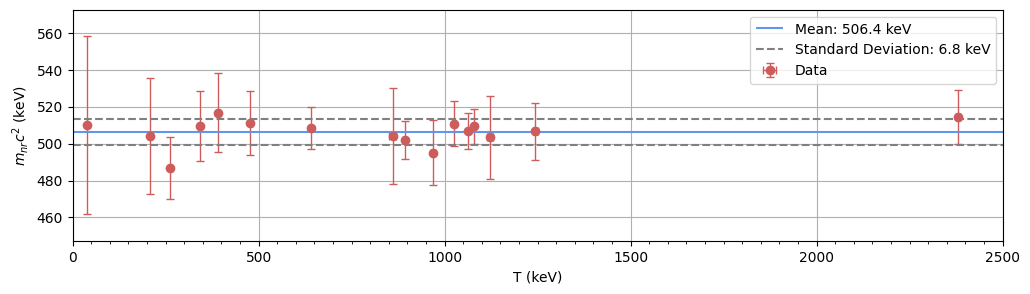
\includegraphics[width=1.7\columnwidth]{relativisticRestMass.png}
				\caption{\label{fig:relativisticRestMass}A graph of the calculations of the rest mass energy using the energies measured from the sources. We see that the rest mass, when treated relativistically, is a constant with respect to the kinetic energy.}
			\end{figure*}		
		
		\subsection{Methodology}
			In this part of the experiment, a germanium semiconducter detector was used to measure the gamma ray energy spectra with higher precision than that of the sodium-iodide detector. As in section II.B.2, the system was calibrated using the same calibration sources. To accurately determine the rest mass of the electron, several sources were used to obtain many data points. 11 radioactive sources were measured as listed in table \ref{tab:restMass} although as some of the sources had multiple photopeaks for different decays, 16 sets of data could be made. For each source, the energy of the photopeak and the Compton edge were recorded along with an uncertainty on both. The uncertainty on these values was controlled by the resolution of the spectrum, and determined to be the full width of the photopeak Gaussian.
			
\begin{table}[]
\resizebox{\columnwidth}{!}{%
\begin{tabular}{@{}llll@{}}
\toprule
Substance & Photopeak (keV) & Compton Edge (keV) & Uncertainty \\ \midrule
Bi137     & 569.79          & 392.05             & 5.06        \\
"         & 1063.73         & 859.96             & 8.45        \\
In116     & 416.57          & 262.94             & 3.37        \\
"         & 1096.92         & 892.65             & 3.38        \\
"         & 1291.91         & 1079.19            & 3.37        \\
Na22      & 511             & 341                & 4.22        \\
"         & 1273.76         & 1062.34            & 3.38        \\
Co57      & 122.31          & 39.65              & 2.53        \\
Mn54      & 834.25          & 639.39             & 3.37        \\
Co56      & 1237.45         & 1025.73            & 4.22        \\
K40       & 1460.08         & 1244.2             & 5.61        \\
Te108     & 2613.66         & 2379.51            & 5.97        \\
Cs137     & 661.66          & 477.27             & 4.51        \\
Ba133     & 356.01          & 208.45             & 5.4         \\
Co60      & 1173.01         & 968.58             & 6.02        \\
"         & 1332.6          & 1120.9             & 8.02        \\ \bottomrule
\end{tabular}%
}
\caption{Table of sources used with their respective measurement for the energy of the photopeak and the Compton edge. Quotation marks in the 'Substance' column denote another photopeak for the same source.}
\label{tab:restMass}
\end{table}



		
		\subsection{Results and Analysis}
			The data from table \ref{tab:restMass} was graphed in figure \ref{fig:classicalRestMass} using the classical formulation of the rest mass, equation \ref{eq:classical} and they were also graphed in figure \ref{fig:relativisticRestMass} using the relativistic formulation of the rest mass, equation \ref{eq:relativistic}. Figure \ref{fig:classicalRestMass} plots the classical representation of the rest mass whereas figure \ref{fig:relativisticRestMass} plots the relativistic representation. Least squares fitting was used to plot a linear line through the data for the classical representation whereas a simple mean and standard deviation were determined and plotted for the relativistic representation. We see that the rest mass energy increases as a function of kinetic energy in the classical approach. Our assumptions to form the classical equations are not sufficient as by definition the rest mass energy should not increase as a function of the kinetic energy. Conversely, in the relativistic approach we see that the rest mass is a constant with respect to the kinetic energy. We can hence conclude that the electrons in these reactions should be treated relativistically and that the assumption to do so made in the calculations of section II of this report are valid.

	\section{Conclusion}
		The overarching aim of this report was to investigate the scattering interaction between gamma rays and electrons known as Compton scattering. The aims were to determine the energy of the gamma ray after the interaction as a function of angle and to determine the differential cross-section. A separate experiment was undertaken to investigate whether the electrons in this interaction need to be treated relativistically or if classical assumptions are sufficient.\\
		
		The gamma ray energy measured as a function of the scattering angle closely followed that of the theoretical function. We see a linear linear function for the reciprocal of the energy which only deviates from the theory by a constant offset. This is likely due to a systematic error in the misalignment of the apparatus. Further experiments to repeat these calculations with different apparatus could be carried out to remove this offset error. We see that the differential cross-section measured follows closely that of the Klein-Nishina formula with the equation falling within the bounds of uncertainty of nearly all the data. The only deviation from the theory is for scattering angles less than 20 degrees where it is likely that incident gamma rays are directly detected and interfere with the results from the scattered rays.\\
		
		We conclude from the second part of this investigation that the electrons involved in Compton scattering should be treated relativistically. By calculating the rest mass energy of the electron as a function of the electron kinetic energy, it was determined that treating them classically results in a linear increase in rest mass energy as a function of the kinetic energy. However when treated relativistically the rest mass energy stays constant as expected.
		
		
	\clearpage
	\bibliography{comptonScattering.bib}% Produces the bibliography via BibTeX.
	
	\clearpage
	\onecolumngrid
	\appendix
	\section{Caesium-137 Spectrum Data}
	
% Please add the following required packages to your document preamble:
% \usepackage{booktabs}
% \usepackage{graphicx}
\begin{table}[H]
\resizebox{\columnwidth}{!}{%
\begin{tabular}{@{}lllllllll@{}}
\toprule
Angle Left & Angle Right & Avg Angle & Energy (keV) & FWHM (keV) & Net Counts & Uncertainty & Live Time & Real Time \\ \midrule
85         & 74.25       & 79.625    & 317.83       & 40.64      & 15837      & 544         & 291.22    & 291.78    \\
80         & 69.25       & 74.625    & 334.51       & 47.58      & 13190      & 492         & 233.34    & 233.8     \\
75         & 64.25       & 69.625    & 353.52       & 50.79      & 10691      & 422         & 175       & 175.38    \\
70         & 59.25       & 64.625    & 372.42       & 42.93      & 10268      & 389         & 159.62    & 160       \\
65         & 54.25       & 59.625    & 395.22       & 56.93      & 11211      & 365         & 148.16    & 148.56    \\
60         & 49.25       & 54.625    & 419.84       & 53.42      & 10695      & 424         & 142.16    & 142.56    \\
55         & 44.25       & 49.625    & 444.27       & 55.75      & 10546      & 413         & 123.58    & 125.86    \\
50         & 39.25       & 44.625    & 467.43       & 62.32      & 16675      & 502         & 173.28    & 176.08    \\
45         & 34.25       & 39.625    & 496.4        & 75.68      & 13302      & 403         & 126.08    & 128.92    \\
40         & 29.25       & 34.625    & 522.44       & 69.37      & 10987      & 332         & 92.9      & 95.28     \\
35         & 24.25       & 29.625    & 547.42       & 64.57      & 11012      & 453         & 94.36     & 96.98     \\
30         & 19.25       & 24.625    & 571.76       & 66.64      & 14872      & 457         & 107.78    & 109.78    \\
25         & 14.25       & 19.625    & 594.79       & 61.57      & 15089      & 440         & 89.82     & 92.68     \\
20         & 9.25        & 14.625    & 616.41       & 61.76      & 17480      & 459         & 82.9      & 85.18     \\ \bottomrule
\end{tabular}%
}
\end{table}

	\section{Python3 Code}
\begin{lstlisting}
import numpy as np
import matplotlib.pyplot as plt
from scipy.optimize import curve_fit
from statsmodels.stats.weightstats import DescrStatsW

# Change default colours to personal colour scheme
import matplotlib as mpl
mpl.rcParams['axes.prop_cycle'] = mpl.cycler(color=["indianred", "cornflowerblue",
 "mediumseagreen", "plum", "sandybrown"]) 

rootPath = r"/home/daraghhollman/main/UCD_PASS_Labs/ComptonScattering"

def LoadFile(path):
    data = np.array(np.loadtxt(path, skiprows=1))
    return data

def DegToRad(deg):
    rad = deg * np.pi / 180
    return rad

def RadToDeg(rad):
    deg = rad / np.pi * 180
    return deg

def LinearFunction(x, m, c):
    return m*x + c
    
def InverseGammaEnergyTheory(x):
    return 1.51 + 1.956 * (x)
    
def EnergyAnglePlot(path):
    data = LoadFile(path)

    anglesDeg = data[:,2]
    anglesRad = [DegToRad(el) for el in anglesDeg]

    energies = data[:,3] # note energies in keV
    energiesError = [el/2 for el in data[:,4]]

    anglesToPlot = [1-np.cos(el) for el in anglesRad]
    energiesToPlot = [1/el for el in energies]
    energiesErrorToPlot = [el/energy**2 for el, energy in zip(energiesError, energies)]
    
    # Experiment
    pars, cov = curve_fit(LinearFunction, anglesToPlot, energiesToPlot)
    xRange = np.arange(np.min(anglesToPlot), np.max(anglesToPlot) + 0.01, 0.01)

    plt.errorbar(anglesToPlot, energiesToPlot, xerr=np.sqrt(np.sin(anglesToPlot)**2 * 
    angleError**2), yerr=energiesErrorToPlot, label="Data", fmt="o", capsize=3, linewidth=1)

    plt.plot(xRange, LinearFunction(xRange, pars[0], pars[1]), label="Linear Fit")

    plt.plot(anglesToPlot, [InverseGammaEnergyTheory(el)/1000 for el in anglesToPlot],
     label="Theory")

    print(pars)
    print(np.sqrt(cov))

    plt.grid()
    plt.legend()
    plt.xlabel("1-cos($\phi$)")
    plt.ylabel("$1/E_\gamma$ keV$^{-1}$")
    
def TheoreticalCrossSection(angle, electronRadius, alpha, solidAngle):
    # The Klein-Nishina formula
    A = (electronRadius**2 / 2) * (1 + np.cos(angle)**2) / 
    (1 + alpha * (1 - np.cos(angle)))**2
    B = 1 + (alpha**2 * (1 - np.cos(angle))**2) / ((1 + np.cos(angle)**2) * 
    (1 + alpha * (1 - np.cos(angle))))

    return A * B
    
def MeasuredCrossSection(sumUnderPhotopeak, countingTime, peakEfficiency, massOfRod, 
atomicNumber, atomicMass, solidAngle, intensity):
    
    avogadrosNumber = 6.0221408e23

    numberOfElectronsInSample = massOfRod * atomicNumber * avogadrosNumber / atomicMass
    
    A = sumUnderPhotopeak / countingTime / peakEfficiency
    B = numberOfElectronsInSample * solidAngle * intensity

    return A / B
    
def SolidAngle(detectorArea, distance):
    return detectorArea / distance**2

def IntrinsicPeakEfficiency(energyMeV):
    return 0.1522 * (energyMeV*10**-3)**-1.1325
    
def CrossSectionPlot(path, scaleConstant):
    data = LoadFile(path)

    electronRadius = 2.82 * 10**-13 # cm
    alpha = 1.29 # For Cs137, Photopeak energy / electron rest mass

    intensty = 1.013 * 10**6 * np.exp(-45.59 / 43.48)

    # Theory
    angleRangeRad = np.arange(0, np.pi / 2, 0.01)
    angleRangeDeg = [RadToDeg(el) for el in angleRangeRad]

    anglesDeg = data[:,2]

    energies = data[:,3]
    energiesError = [el/2 for el in data[:,4]]

    netCounts = data[:,5]
    netCountsUncertainty = data[:,6]

    liveTime = data[:,7]

    errors = []
    i = 0
    for el in netCountsUncertainty:
        
        A = el**2*MeasuredCrossSection(1, liveTime[i], IntrinsicPeakEfficiency(energies[i]), 
        79.3, 13, 26.98, solidAngle, intensty)**2
        B = (energiesError[i]/2)**2 * (-0.1724*(energies[i]*10**-3)**-2.1325 * 10**-3)**2 *\
              (-netCounts[i] / ((79.3 * 13 * 6.022e23 / 26.98) * solidAngle *
               IntrinsicPeakEfficiency(energies[i])**2 * liveTime[i] * intensty))**2
        
        errors.append(scaleConstant * np.sqrt(A + B))
        
        i+=1


    plt.errorbar(anglesDeg, scaleConstant * MeasuredCrossSection(netCounts, liveTime, 
    IntrinsicPeakEfficiency(energies), 79.3, 13, 26.98, solidAngle, intensty),\
             fmt="o", label="Data", xerr=RadToDeg(angleError), yerr=errors, linewidth=1, 
             capsize=3)
    
    plt.plot(angleRangeDeg, TheoreticalCrossSection(angleRangeRad, electronRadius, alpha, 
    solidAngle), label="Theory: Klein-Nishina")
    
    plt.grid()
    plt.xlabel("Scattering Angle (Degrees)")
    plt.ylabel("Differential Cross Section (cm$^2$/sr)")
    plt.legend()
    
def ClassicalRestMass(gammaEnergy, kineticEnergy):
    return 0.5 * (2*gammaEnergy - kineticEnergy)**2 / kineticEnergy

def RelativisticRestMass(gammaEnergy, kineticEnergy):
    return 2 * gammaEnergy * (gammaEnergy - kineticEnergy) / kineticEnergy
    
def UnpackComptonRealtivisticData(path):
    data = LoadFile(path)

    photopeaks = data[:,0]
    comptonEdges = data[:,1]
    uncertainty = data[:,2]

    return [photopeaks, comptonEdges, uncertainty]
    
def ClassicalRestEnergyPlot(path):

    photopeaks, comptonEdges, uncertainties = UnpackComptonRealtivisticData(path)

    restMasses = [ClassicalRestMass(photopeak, comptonEdge) for photopeak, comptonEdge in\
     zip(photopeaks, comptonEdges)]

    pars, cov = curve_fit(LinearFunction, comptonEdges, restMasses)

    yError = [np.sqrt(((T**2 - 4 * E**2) / (2 * T**2))**2 * u**2) for E, T, u in\
     zip(photopeaks, comptonEdges, uncertainties)]

    plt.errorbar(comptonEdges, restMasses, yerr=yError, zorder=2, label="Data", fmt="o",\
     linewidth=1, capsize=3)

    plt.plot(comptonEdges, LinearFunction(comptonEdges, pars[0], pars[1]),\
     color="cornflowerblue", zorder=1, label="Linear Fit")

    plt.grid()
    plt.xlabel("T (keV)")
    plt.ylabel("$m_{nr} c^2$ (keV)")
    plt.legend()
    
def RelativisticRestEnergyPlot(path):
    
    plt.figure(figsize=(12,3))

    photopeaks, comptonEdges, uncertainty = UnpackComptonRealtivisticData(path)

    restMasses = [RelativisticRestMass(photopeak, comptonEdge) for photopeak, comptonEdge in\
     zip(photopeaks, comptonEdges)]

    yError = [np.sqrt((2 * E**2 / T**2)**2 * u**2) for E, T, u in zip(photopeaks, \
    comptonEdges, uncertainty)]

    plt.errorbar(comptonEdges, restMasses, xerr=uncertainty, yerr=yError, fmt="o",\
     linewidth=1, capsize=3, zorder=2, label="Data")

    stats = DescrStatsW(restMasses, weights=[error/np.min(yError) for error in yError],\
     ddof=0)

    mean = stats.mean
    std = stats.std

    plt.hlines(mean, 0, 2500, color="cornflowerblue", linestyles="-", label=f"Mean: \
    {mean:.1f} keV")
    plt.hlines(mean+std, 0, 2500, color="grey", linestyles="--", label=f"Standard Deviation: \
    {std:.1f} keV")
    plt.hlines(mean-std, 0, 2500, color="grey", linestyles="--")

    plt.xlabel("T (keV)")
    plt.ylabel("$m_{nr} c^2$ (keV)")
    plt.legend()
    plt.xticks(np.arange(0, 2501, 500))
    plt.xticks(np.arange(0, 2501, 50), minor=True)
    plt.margins(x=0, y=0.15)
    plt.grid()

\end{lstlisting}

		
\end{document}

